\subsection{The current conveyor as a multiplier}

\begin{figure}[H]
    \centering
    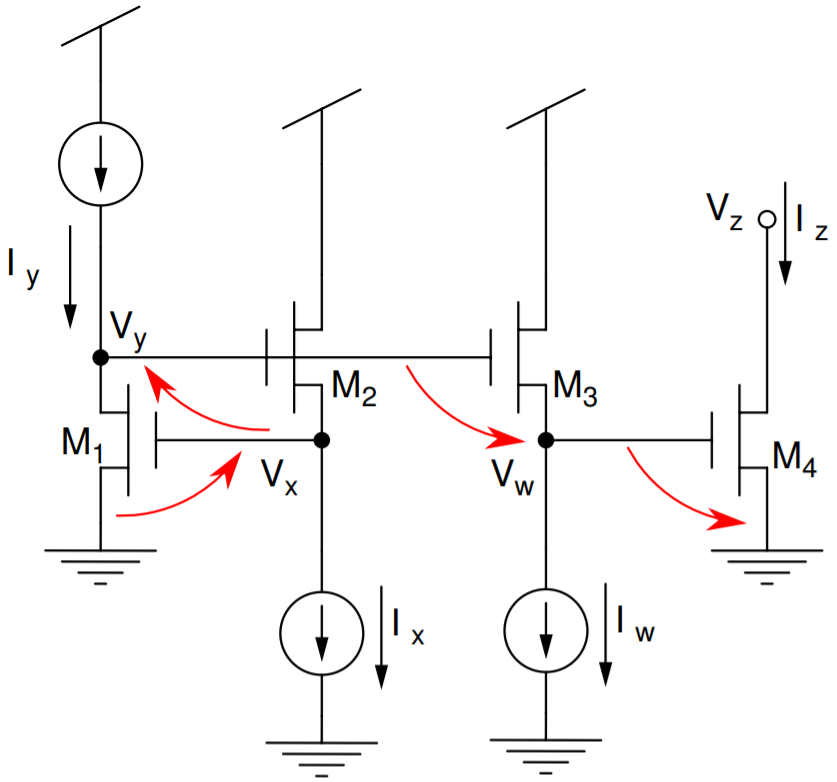
\includegraphics[width=0.5\linewidth]{../../Figures/Current_Multiplier.PNG}
    \caption{Current conveyor as a multiplier. Adapted from Lecture notes.}
    \label{fig:Current_Multiplier}
\end{figure}

Let's look at what this circuit does. The first thing to notice is that building block (on the left) is exactly the current conveyor we've seen before, with $I_x$, $I_y$ and $I_z$ etc. Now, let's look at the $V_{gs}$'s, remembering the translinear principle. Look at the red arrows represent the $V_{gs}$ of each transistor: two of them (on the left) go \textit{from} ground and the two others (on the right) go \textit{into} ground. Yes! The translinear principle applies. Let's put that formally: 

\begin{itemize}
    \item First $V_{gs_1} = V_x - 0$
    \item Second $V_{gs_2} = V_y - V_x$
    \item Third $V_{gs_3} = V_y - V_w$
    \item Fourth $V_{gs_4} = V_w - 0$
\end{itemize}

Applying the translinear principle, this yields: 

\begin{equation}
    (V_x - 0) + (V_y - V_x) - (V_y - V_w) - (V_w - 0) = 0
\end{equation}
\begin{equation}
    \rightarrow V_{gs_1} + V_{gs_2} - V_{gs_3} - V_{gs_4} = 0
\end{equation}
\begin{equation}
    \rightarrow I_x \cdot I_y \cdot {I_w}^{-1} \cdot {I_z}^{-1}= 0
\end{equation}
\begin{equation}
    \mathrm{Yielding \ the \ elegant: }\ I_z = \frac{I_x \cdot I_y}{I_w} 
\end{equation}

One must remember that this is an approximation as we assumed in the translinear principle derivation earlier that $\kappa = 1$, which is not true in practice. As a reminder, $\kappa$ is usually ~0.7-0.8 in practice.  




